\chapter{Metodologia}
% Label para referenciar
\label{metodologia}
O estudo apresenta a modelagem e desenvolvimento de uma arquitetura que possibilite a extração, processamento e disponibilização dos dados referente à Câmara dos Deputados Federal. Este projeto foi desenvolvido utilizando a plataforma Databricks, que pode ser definida como uma plataforma unificada para análise de dados na \textit{Cloud} para um volume massivo de dados, promovendo a colaboração entre Cientistas e Engenheiros de Dados\footnote{Disponível em <https://databricks.com/product/unified-data-analytics-platform> Acesso em: 19 mai, 2020}.
A arquitetura pode ser definida em 3 camadas (serão detalhadas nas seções a seguir):
\begin{enumerate} 
 \item [1)] Armazenamento;
 \item [2)] \textit{Extract, Transform and Load (ETL)};
 \item [3)] Análise exploratória de dados.
\end{enumerate} 

Pode-se ter uma visão mais detalhada na imagem abaixo.

% Figura
\begin{figure}[!ht]
	\centering	
	\caption[\hspace{0.1cm}Arquitetura proposta]{Arquitetura proposta}
	  \vspace{-0.4cm}
	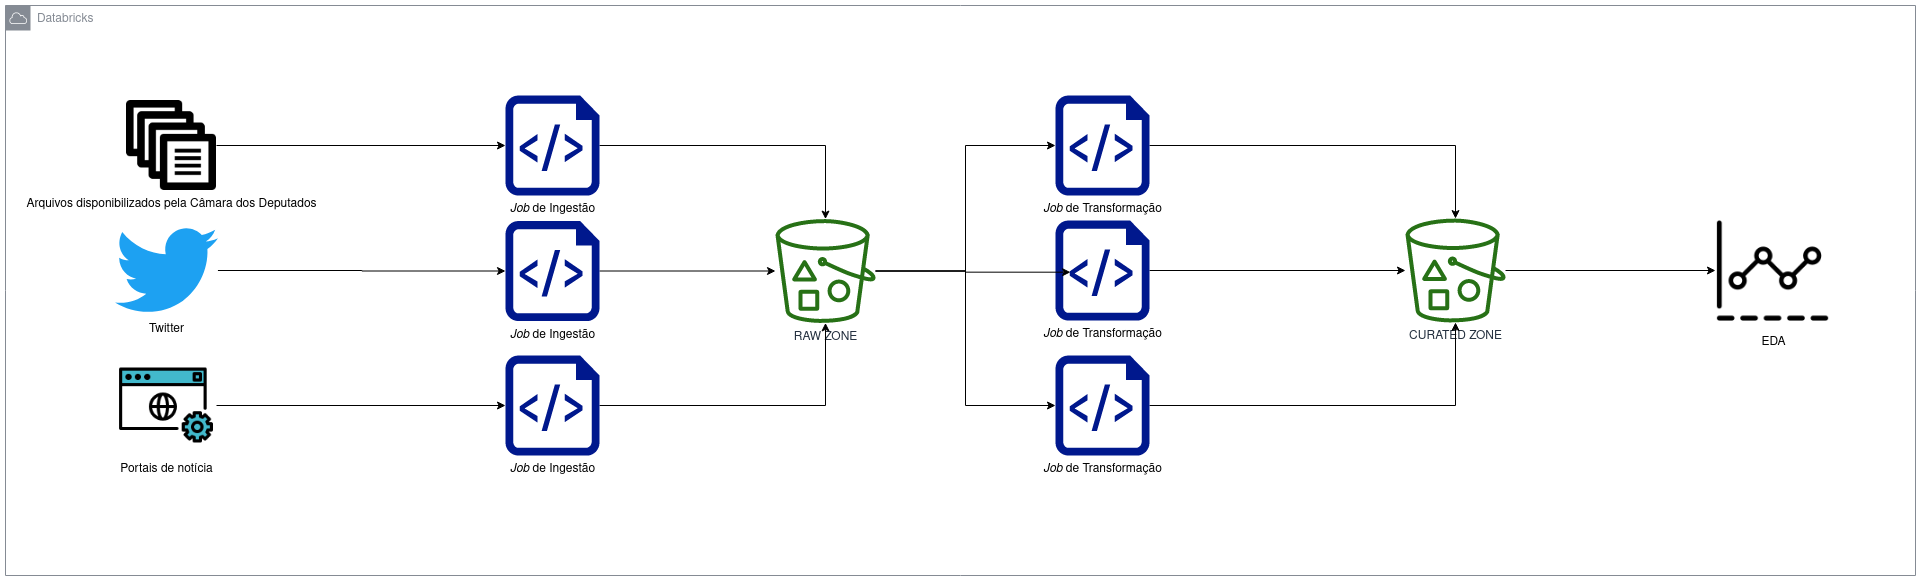
\includegraphics[width=.8\textwidth]{figuras/tcc_arch.png}
	% Caption centralizada
% 	\captionsetup{justification=centering}
	% Caption e fonte
	 \vspace{-0.3cm}
	\\\textbf{\footnotesize Fonte: Elaborada pelos autores}
	\label{fig:tela1}
\end{figure}

\section{Armazenamento} Como descrito no início do capítulo, o Databricks está sendo utilizado como plataforma unificada do projeto, o que inclui o seu armazenamento. O Databricks oferece um \textit{file system} distribuído para o armazenamento de dados em sua plataforma. É denominado como \textit{Databricks File System (DBFS)} e é compartilhado por todos os nós do \textit{cluster}\footnote{Disponível em <hhttps://docs.databricks.com/data/databricks-file-system.html> Acesso em: 19 mai, 2020}. Uma arquitetura de \textit{Data Lake} está sendo utilizada, logo temos a segmentação dos dados em zonas. Os dados originais são armazenados na zona \textit{RAW} em seu formato original. Após os processos de ETL, os dados já tratados são armazenados na zona \textit{CURATED} em formato parquet, uma vez que esse formato de armazenamento colunar é otimizado para o uso com o Spark e diminui drasticamente o espaço em disco necessário\footnote{Disponível em <https://parquet.apache.org/> Acesso em: 19 mai, 2020}.

\section{\textit{Extract, Transform and Load (ETL)}} Todo o processamento deste projeto foi realizado utilizando o Apache Spark. Este processamento foi segmentado em duas etapas, sendo elas:

\subsection{Ingestão de dados} Essa camada tem como objetivo o detalhamento dos processos que extraem os dados de sua fonte originária e os inserem, sem maiores tratamentos, no ambiente analítico. Foram elencadas 3 fontes de dados para o projeto. Iremos descrever abaixo as características de cada uma.

\subsubsection{Dados Abertos da Câmara dos Deputados} A fonte oficial de dados da Câmara dos Deputados. Se trata de arquivos históricos disponibilizados pelo Câmara que contém todas as informações pessoais e políticas dos parlamentares, além de seu histórico de reembolsos, discursos políticos, votações, emendas de sua autoria ou co-participação, entre diversas outras informações referentes à sua atividade parlamentar\footnote{Disponível em <https://dadosabertos.camara.leg.br/> Acesso em: 19 mai, 2020}. Os arquivos de 2009 à 2019 foram extraídos manualmente e inseridos na zona \textit{RAW} do nosso \textit{Data Lake}. Para esse projeto, os dados dos seguintes temas foram extraídos:

\begin{itemize}
\item \textbf{Dados dos Deputados}: Listagem de todos os deputados que já estiveram em exercício na Câmara dos Deputados;
\item \textbf{Despesas dos parlamentares}: Listagem de todas as despesas referentes ao exercício da Atividade Parlamentar de cada deputado;
\item \textbf{Proposições}: Listagem de todas as proposições apresentadas à Câmara dos Deputados com suas respectivas informações;
\item \textbf{Autores das Proposições}: A listagem de todos os autores das proposições submetidas à Câmara;
\item \textbf{Classificação temática das proposições}: Informações mais detalhadas referentes aos temas das proposições submetidas.
\end{itemize}

\subsubsection{API do Twitter} O Twitter é uma rede social criada em 15 de julho de 2006 e, em fevereiro de 2019, possuia 321 milhões de usuários ativos\footnote{Disponível em <https://pt.wikipedia.org/wiki/Twitter> Acesso em: 19 mai, 2020}.Para extrair os \textit{tweets} desta plataforma, foi criado um \textit{job} utilizando Python e um módulo de comunicação com Twitter, o tweepy, que é caracterizado pelos autores como uma biblioteca de fácil uso para acesso à API do Twitter\footnote{Disponível em <https://www.tweepy.org/> Acesso em: 19 mai, 2020}. Para esse projeto, um arquivo com a listagem de todos os deputados e seus respectivos perfis oficiais no Twitter foi preenchido manualmente. Dessa forma, tornou-se possível a extração de todas as publicações de autoria dos parlamentares na plataforma.

\subsubsection{Portais de notícia} Se tratando dos portais de notícia, foi elencado o portal G1 como fonte de notícias políticas para alimentar o ambiente analítico. Para esse fim, um \textit{job} em Spark foi desenvolvido para realizar a extração das notícias políticas. Um filtro será utilizado para extrair somente os artigos que tenham alguma referência aos parlamentares. 

\subsection{Transformação dos Dados} Nesta etapa, a limpeza e estruturação dos dados é realizada. Os dados armazenados na zona \textit{RAW} são utilizados como \textit{input} para essa camada da \textit{pipeline}. O processamento pode ser resumido na limpeza dos dados, filtro das informações e a estruturação das entidades para que a Análise Exploratória seja possível posteriormente. Após esse tratamento, os dados são armazenados em formato parquet na zona \textit{CURATED}. Vários arquivos são escritos nessa zona em \textit{folders} que tem a finalidade de abstrair essas entidades. Essa zona segue a seguinte estrutura:

% Figura
\begin{figure}[H]
	\centering	
	\caption[\hspace{0.1cm}Zona Curated]{\textit{Curated zone}}
	  \vspace{-0.4cm}
	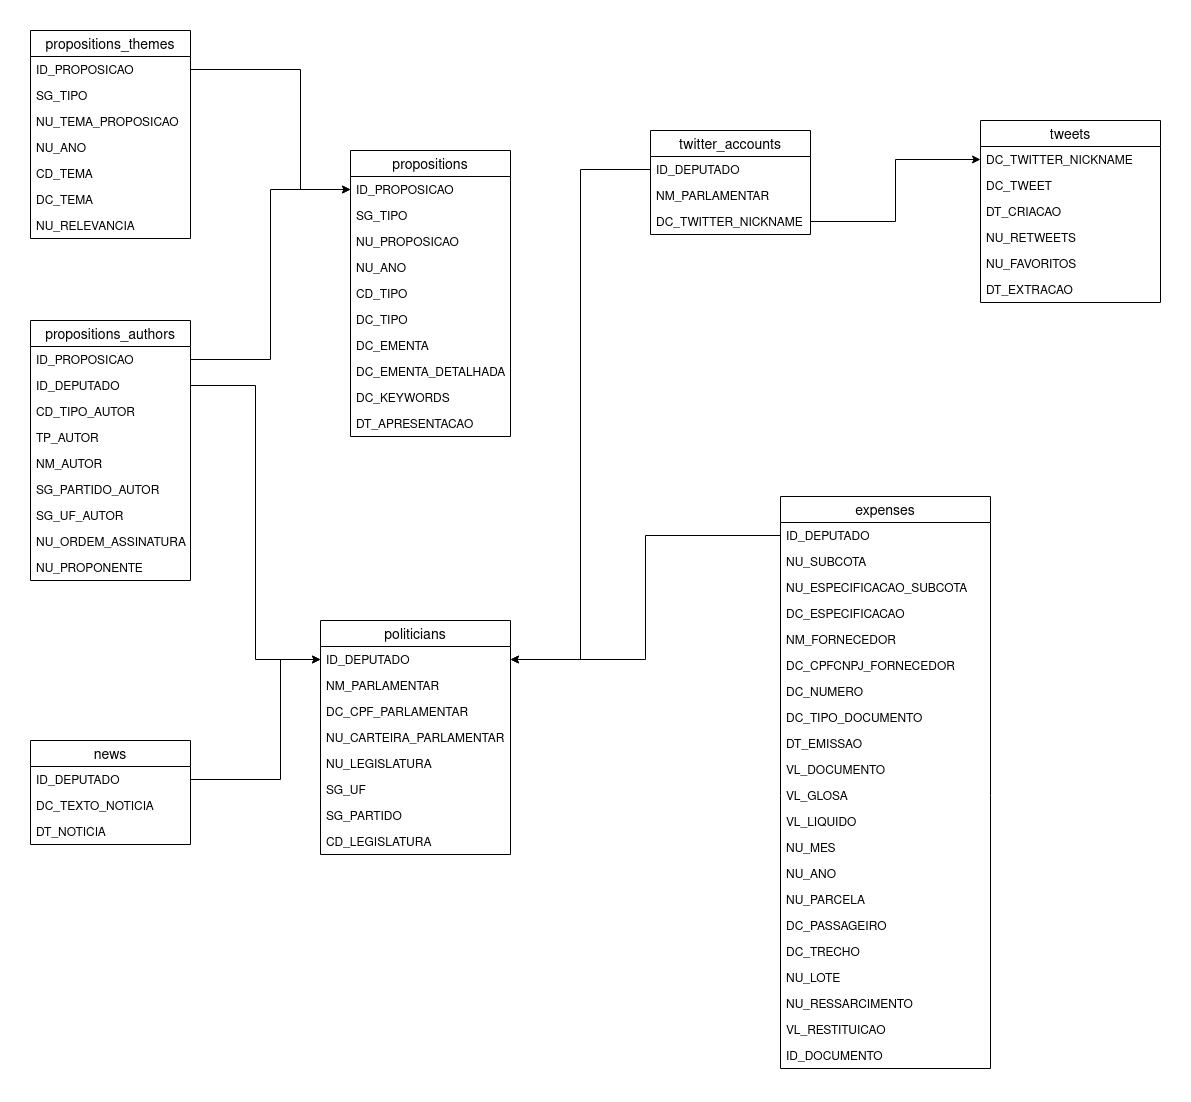
\includegraphics[width=.8\textwidth]{figuras/er_tcc.png}
	% Caption centralizada
% 	\captionsetup{justification=centering}
	% Caption e fonte
	 \vspace{-0.3cm}
	\\\textbf{\footnotesize Fonte: Elaborada pelos autores}
	\label{fig:tela1}
\end{figure}

\section{Análise exploratória de dados} A Análise exploratória de dados, também conhecida no campo da Estatística como \textit{Exploratory Data Analysis (EDA)} consiste na etapa de exploração dos dados em busca de padrões. Conforme descrito nas seções anteriores, todos os passos para extração e limpeza dos dados já foram realizados e, utilizando a \textit{Curated Zone}, os dados estão prontos para análise.